% 1977 年湖南株洲卷第 10 题：山顶 P 处测正南两船 A、B 的俯角 15° 与 75°，
% PC 铅垂高 150m，DP 为过 P 的水平线（虚线），PA、PB 为视线（虚线）（按源卷第 5 页布局）
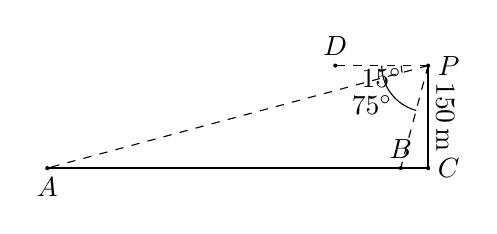
\begin{tikzpicture}[scale=0.62]
  \coordinate (P) at (0,0);
  \coordinate (D) at (-1.9,0);
  \coordinate (C) at (0,-2.1);
  \coordinate (B) at (-0.56,-2.1);
  \coordinate (A) at (-7.8,-2.1);
  \draw[thick] (A)--(C);
  \draw[thick] (C)--(P);
  \draw[dashed] (P)--(D);
  \draw[dashed] (P)--(A);
  \draw[dashed] (P)--(B);
  \draw ([shift=(180:0.55)]P) arc (180:195.2:0.55);
  \draw ([shift=(180:0.95)]P) arc (180:255.2:0.95);
  \node at (-0.95,-0.25) {$15^\circ$};
  \node at (-1.15,-0.80) {$75^\circ$};
  \fill (P) circle (1.2pt) node[right] {$P$};
  \fill (D) circle (1.2pt) node[above] {$D$};
  \fill (A) circle (1.2pt) node[below] {$A$};
  \fill (B) circle (1.2pt) node[above] {$B$};
  \fill (C) circle (1.2pt) node[right] {$C$};
  \node[rotate=-90] at (0.35,-1.05) {$150\,\mathrm{m}$};
\end{tikzpicture}
